\entry{Semana del 14/07/2025} 
\subsection*{Notas del día:}
\begin{itemize}
	\item Parece que medir el canal 1 sin el 0 da ruido. 
	\item El ajustador está funcionando, pero da con el sensor sumergido 56 kHz de resonancia y debería dar tipo 52 kHz. Filtrando y sacando el ruido sigue dando ahí el máximo de amplitud, y en tiempo real tanto fase 0 rad como máximo de amplitud dan más cerca de 52 kHz. 
	\item Lo mejor será o conectar el generador o la placa como generador a la compu imagino para hacer el barrido punto a punto y ajustar eso que no va a tener casi ruido.  
	
	\item  No parece haber correlación en el ruido del generador de funciones. 
	
	\item Haciendo barrido de frecuencia y analizando de ventanas también da 56 kHz la resoanncia del sistema. Por ahí los barridos son muy rápidos, varío 90 kHz en 1 s. 
	
	\item Por ahí a lo largo de los varios minutos que dura la calibración se forman burbujas que van disminuyendo la superficie del alambre de cobre en contacto con el agua y eso hace que se vaya corriendo la calibración. 
	
\end{itemize} 

\subsection*{Ruido blanco.} 
Seguí completando los métodos para determinar rápidamente la frecuencia de resonancia. Para el ruido blanco usé lo que ya tenía (reduciendo el código para que tome los datos y los analice directamente en vez de guardarlos y analizarlos a parte) y simplemente agregué que se ajuste la respuesta en frcuencias por una Lorentziana con un offset vertical:

\begin{equation}
	A(f) = \frac{A_0}{\sqrt{1 + Q^2 \left(\frac{f}{f_0}-\frac{f_0}{f}\right)^2}} + B 
\end{equation}

Donde $Q$ va a ser el factor de calidad y $f_0$ la frecuencia de resonancia. En general el método parece funcionar bastante bien, lo único que no me convence es que la frecuencia de resoanncia praece estar corrida (da cerca de 56 Khz y debería dar 52 kHz según los métodos previos que venía usando). 

\begin{figure}[th!]
	\centering
	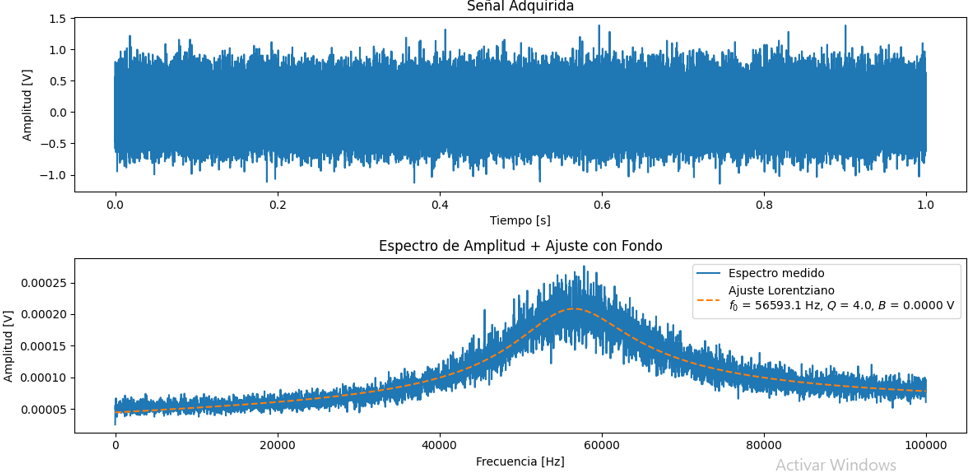
\includegraphics[width=0.87\linewidth]{Figures/14_07_2025/Ajuste_ruido_balnco}
	\caption{Ajuste de la respuesta en frecuencia del RLC serie con el sensor sumergido al ruido blanco por una Lorentiziana.}
	\label{fig:ajusteruidobalnco}
\end{figure}


Cuando traté de suavizar la respuesta en frecuencia tomando más tiempo para Welch o usando más overlap entre ventanas da lo mismo. Me fijé si el ruido del generador estaba correlacionado (y se iba repitiendo) pero no parece ser el caso. 

\begin{figure}[th!]
	\centering
	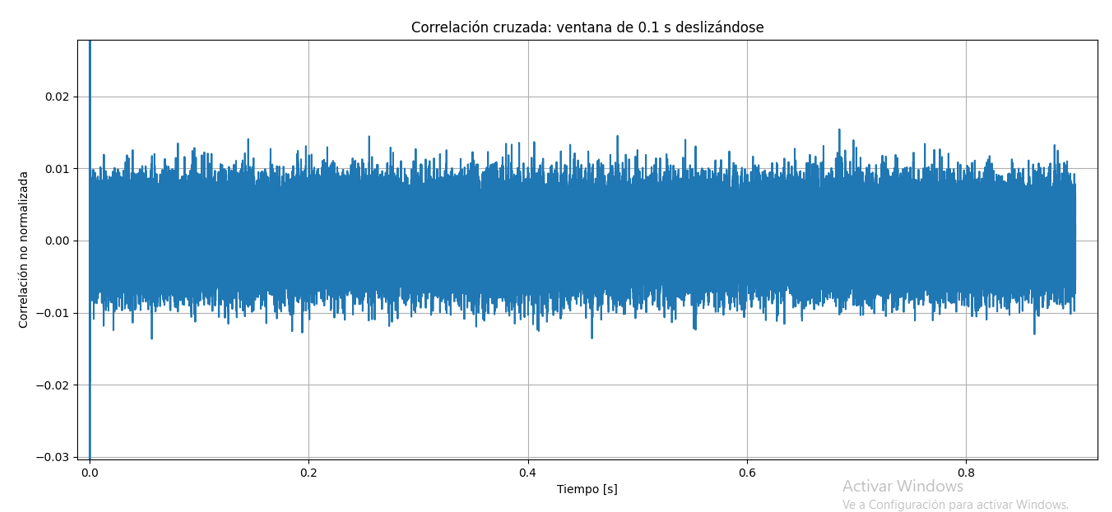
\includegraphics[width=0.7\linewidth]{Figures/14_07_2025/Correlación_ruido}
	\caption{Autocorrelación del ruido del generador de funciones con ventana deslizante.}
	\label{fig:correlacionruido}
\end{figure}


Además se puede suavizar alternativamente la respuesta usando algún filtro. Ya sea un moving average (pero esto corre para la derecha todaví más la campana de resonancia) o Savot-Golay que mantiene la posición del pico, obteniendo muy buenos resultados. 

\subsection*{Sweep en frecuencia con el generador.} %,  
Después por último intenté configurar el generador de funciones en modo sweep (barrido lineal de frecuencias en un tiempo determinado) y analizar la medición por ventanas, tomando la frecuencia instantánea con Hilbert y la amplitud y fase con Lock-in. Esto también pareció funcionar bastante bien, pero la frecuencia sigue estando corrida, por ahí estos métodos son demasiado rápidos y por eso se desplaza la frecuencia de resonancia, en función de lo que tarda en responde el circuito. 

\begin{figure}[th!]
	\centering
	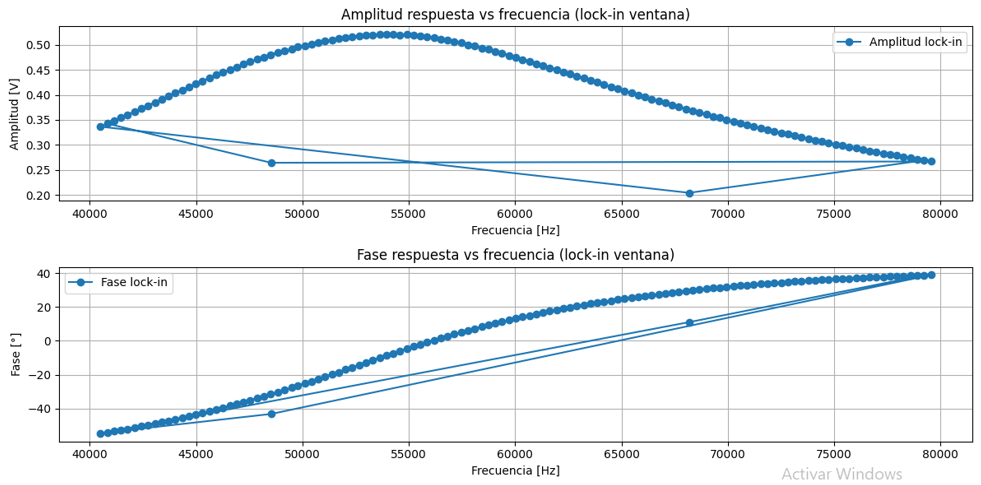
\includegraphics[width=0.87\linewidth]{Figures/14_07_2025/Sweep_generador_Hilbert_plus_Lockin}
	\caption{Amplitud y fase para sweep con el generador de funciones analizando por ventana.}
	\label{fig:sweepgeneradorhilbertpluslockin}
\end{figure}



\section{Miércoles 16/07/2025.}
\subsection*{Notas del día:}
\begin{itemize}
	\item Empiezo calibrando con una rampa de amplitud de 0 a 10 mm con frecuencia 52.270 kHz. Tomé 40 segundos de datos, la rampa ida y vuelta toma un total de 10 segundos. 
	\item Voy a hacer lo mismo pero más rápido. Ahora 5 segundos por rampa completa. Para esta frecuencia de 52.040 kHz. 
	
	\item Ahora voy a aprobar otras cosas. En particular quiero un forzado típico de turbulencia de ondas y algún con frecuencias más altas. 
	\item Esta tocando el borde de la tapa el alambre de acero. Parece que 10 segundos es muy rápido y se empieza a formar Faraday tal vez. 
	\item Ahora intento lo mismo pero durando 40 segundos el forzado. Ambos con frecuencia de corriente de 52.050 kHz. Tenía demasiada amplitud así que no lo hice. 
	
	\item Lo hago par máx 1 Hz en el espectro para 10 y 40 s. El agua vibra por el motor en cualquier caso parece ser. 
	
	\item Por último de nuevo la rampa pero ahora de -10 a 10 en 1 s. Vibra mucho. Ya 40 s sería demasiado tiempo, probé máximo 10 segundos ida y vuelta completa. 
\end{itemize} 

\subsection*{Calibración con el wavedriver - Montaje.} 
Hoy ya sí monté para calibrar el sensor con el Wave - Driver. Básicamente con se ve en la foto tengo montado en uno de los perfiles de la cuba el motor vertical con uno de los soportes que hicimos el año pasado paar los toroides, cuyo tamaño era perfecto para que entrase un recipiente con agua destilada (la tapita del spray aislante). Luego tengo sobre la mesa el sensor sobre su soporte común de perfiles de aluminio. 

El procedimiento que estoy usando para medir es el siguiente: Primero hago el homing, después doy a que empiece la curva que tiene precargada el motor y recién ahí agrego el recipiente con agua (o como mucho antes justo después del homing) y coloco el sensor para asegurarme de que no choque con el fondo. Para esto tuve que probar distintos homings y usar el tornillo para el ajuste final. La tapa tendría un par de centímetros de agua destilada. 




\section{Jueves 17/07/2025.}
Hoy prendí la Compu a la tarde y la pantalla tenía los colores raros, como si faltase el canal rojo, la llevamos a arreglar, así que pauso el análisis hasta entonces. 

\section{Viernes 18/07/2025.} 
Parece que la placa de atrás de la pantalla era el problema, terminaron cambiando la pantalla entera pero para última hora de hoy ya tuve la Compu de nuevo. 